\chapter{Modelli teorici}\label{ch:modelli}
Nel capitolo precedente si è visto che tra i principali obiettivi fisici dell'esperimento ALICE c'è lo studio del QGP e della transizione da questo stato alla materia ordinaria.
Questa transizione è descritta da diversi modelli teorici in cui la formazione di adroni a partire da quark singoli viene implementata utilizzando processi fisici e formalismi differenti. 
Due modelli largamente utilizzati sono il modello di coalescenza e quello di adronizzazione statistica.

In questo capitolo verranno esposti questi due modelli e verranno effettuati dei confronti tra essi.
Inoltre verrà introdotto il generatore Monte Carlo \pythiaa{} \cite{pythia8300}, nel quale si utilizza un altro modello di formazione basato sul processo di frammentazione di stringa, ossia il modello di sezioni d'urto efficaci. 

\section{Il modello di coalescenza}
Nel modello di coalescenza, i nucleoni generati dalla collisione vanno a formare un nucleo se essi sono vicini nello spazio delle fasi.
Per comprendere meglio, il modello si incentra su un parametro $B_A$, detto \emph{di coalescenza}, il quale è un indicatore della probabilità di formazione del nucleo.
Esso è definito nel seguente modo \cite{alice_2022_coal_formula}:
\begin{equation}\label{eq:coal}
    \dfrac{1}{2\pi p_t^\text{A}}\dfrac{d^2N_\text{A}}{dy\ dp_t^\text{A}} = B_\text{A}({p_t}^\text{p}) \cdot  \left(\dfrac{1}{2\pi p_t^\text{p}}\dfrac{d^2N_\text{p}}{dy\ dp_t^\text{p}}\right)^A
\end{equation}
con p e A che si riferiscono ai (anti)protoni e ai (anti)nuclei con numero di massa $A$, $p_t$ la quantità di moto trasversa del nucleo, $N_p$ e $N_A$ il numero di (anti)protoni e (anti)nuclei rispettivamente.
Il significato dell'\autoref{eq:coal} è il seguente: il membro a sinistra indica gli spettri invarianti di produzione dei (anti)nuclei, mentre il termine a destra è il prodotto tra $B_A$ e gli spettri invarianti di (anti)protoni.\\

Inizialmente il modello di coalescenza si basava su un modello fenomenologico: qualsiasi coppia (anti)protone-(anti)neutrone forma un (anti)deuterone nel momento in cui il modulo della differenza della loro quantità di moto ($|\vec p_p - \vec p_n|$) è minore di un parametro costante $p_0$.
Quindi il processo non è probabilistico, ma deterministico e indipendente dalle dimensioni del sistema considerato e dalla distanza che separa i nucleoni.
Per questo motivo questo modello viene chiamato \emph{modello semplice}.
Questo modello è valido sperimentalmente solamente per le collisioni che prevedono sistemi con dimensioni ridotte, come per esempio le collisioni p-nucleo, mentre per i sistemi più estesi, si osserva sperimentalmente una dipendenza con le dimensioni del nucleo.
Questo modello è utilizzato soprattutto per i simulatori Monte Carlo poiché i meccanismi di formazione sono semplici da gestire.\\

Un modello più adeguato dovrebbe considerare anche le dimensioni del nucleo e che due nucleoni vicini nello spazio dei momenti non necessariamente formano un nucleo, seguendo un approccio stocastico che rispecchi la natura quantomeccanica del processo.
Per avere una descrizione più rigorosa, si utilizzano le funzioni di Wigner per la rappresentazione dello spazio di fase del nucleo \cite{Scheibl_1999_wigner}.
Per esempio nel caso più semplice, quello del deuterone, una possibile funzione d'onda del deuterone può essere scritta sotto forma di una gaussiana, 
\begin{equation}
    \phi_D(\vec r) = (\pi {r_D}^2)^{-3/4}\ \exp\left(\dfrac{-r^2}{2{r_D}^2}\right)
\end{equation}
con $r_D$ il raggio caratteristico del deuterone.

Considerando la natura quantomeccanica delle particelle, è necessario aggiungere un fattore di correzione medio \cite{Scheibl_1999_wigner}.
Questo è definito come
\begin{equation}
    \lrangle{C_A} = \prod_{i=1,2,3}\left(1+\dfrac{r^2}{4R_i^2}\right)^{-\frac{A-1}2}
\end{equation}
con $R_i$ la proiezione del raggio sull'asse $x_i$.
Assumendo un'approssimazione isotropica della sorgente, allora si può dimostrare che il parametro di coalescenza assume la seguente espressione
\begin{equation}
    B_A = \dfrac{2J_A+1}{2^A}\dfrac{1}{\sqrt{A\ m_T^{A-1}}} \left(\dfrac{2\pi}{R^2 + \left(\frac{r_A}{2}\right)^2}\right)^{\frac32(A-1)}
\end{equation}
con $J_A$ e $r_A$ lo spin e il raggio caratteristico del nucleo, $m_t = \sqrt{m^2+p_t^2}$ la massa trasversa e $R$ la dimensione caratteristica della sorgente.
Questa espressione ha senso perché tiene conto sia delle dimensioni della sorgente che di quella del nucleone.
È importante notare che il parametro $B_A$ non dipende solamente dal numero di massa, ma anche dalla specie considerata.
Per esempio se si tiene in conto $^{3}{\rm He}$ e $^{3}{\rm H}$, essi differiscono per il parametro $r_A$, in particolare $r_{^{3}{\rm He}} =  2.48$ fm e $r_{^{3}{\rm H}} = 2.15$ fm \cite{PURCELL20151_nuclear_sheet}.\\

Per mostrare la validità di questo modello si esegue un confronto tra dati di ALICE e le previsioni del modello esposto.
In particolare si confrontano le funzioni dei parametri di coalescenza $B_2$ e $B_3$ in funzione della molteplicità \cite{alice_2022_coal_formula} (\autoref{fig:BAvsMult}).
Per gli andamenti teorici si utilizzano due parametrizzazioni: il primo ("A") è basato sul fit ai dati sperimentali di ALICE del raggio del sistema (effettuato con misurazioni femtoscopiche, \cite{PhysRevD.87.052016_femto}) in funzione della molteplicità; mentre nella seconda ("B") la relazione tra il raggio del sistema e la molteplicità viene fissata per riprodurre il $B_2$ dei deuteroni in collisioni Pb-Pb a una energia nucleone-nucleone $\sqrt{s_{NN}} = 2.76$ TeV.
\begin{figure}[h]
    \centering
    \begin{subfigure}{.49\textwidth}
    \centering
        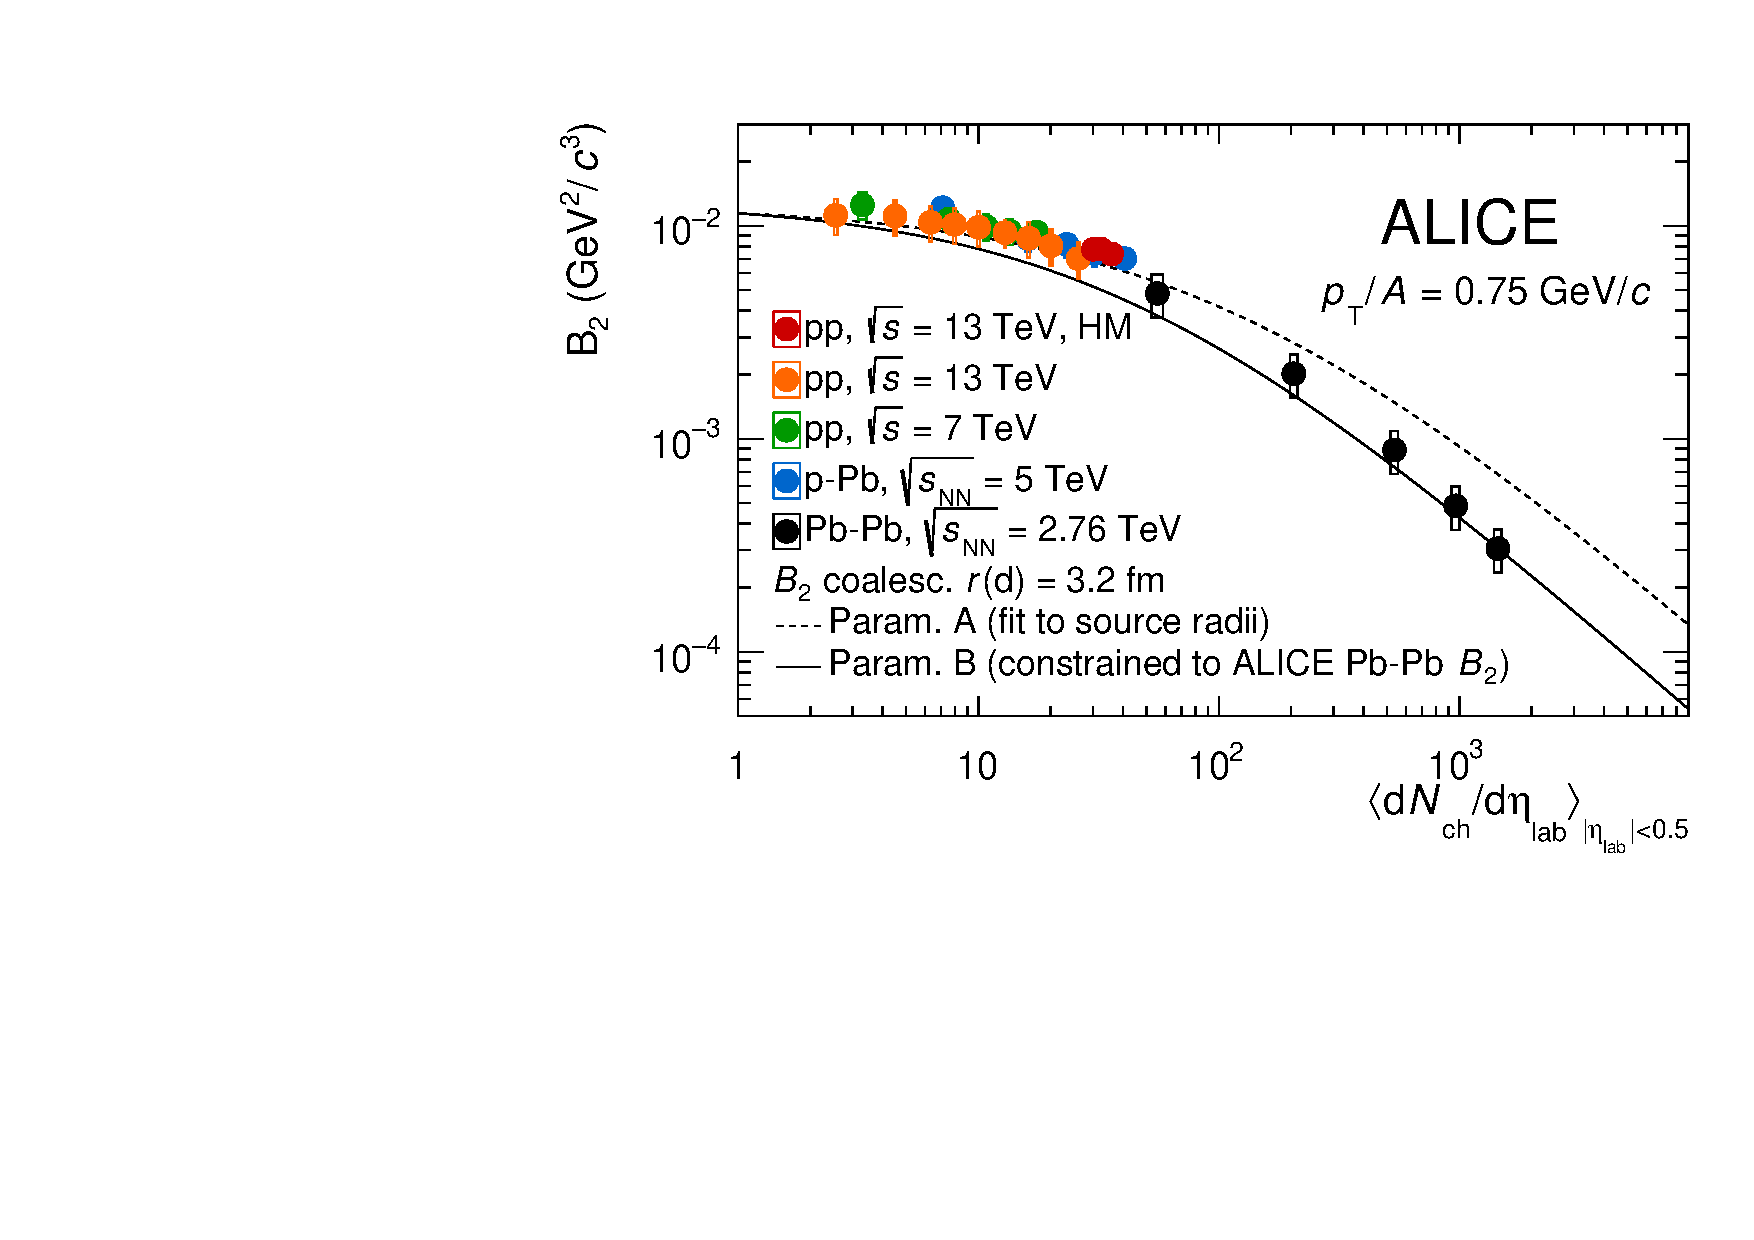
\includegraphics[width=\textwidth]{image/2-modelli/cB2vsMult.pdf}
        \caption{(Anti)deuteroni}
        \label{fig:cB2vsMult}
    \end{subfigure}
    %\hspace{1cm}
    \begin{subfigure}{.49\textwidth}
        \centering
        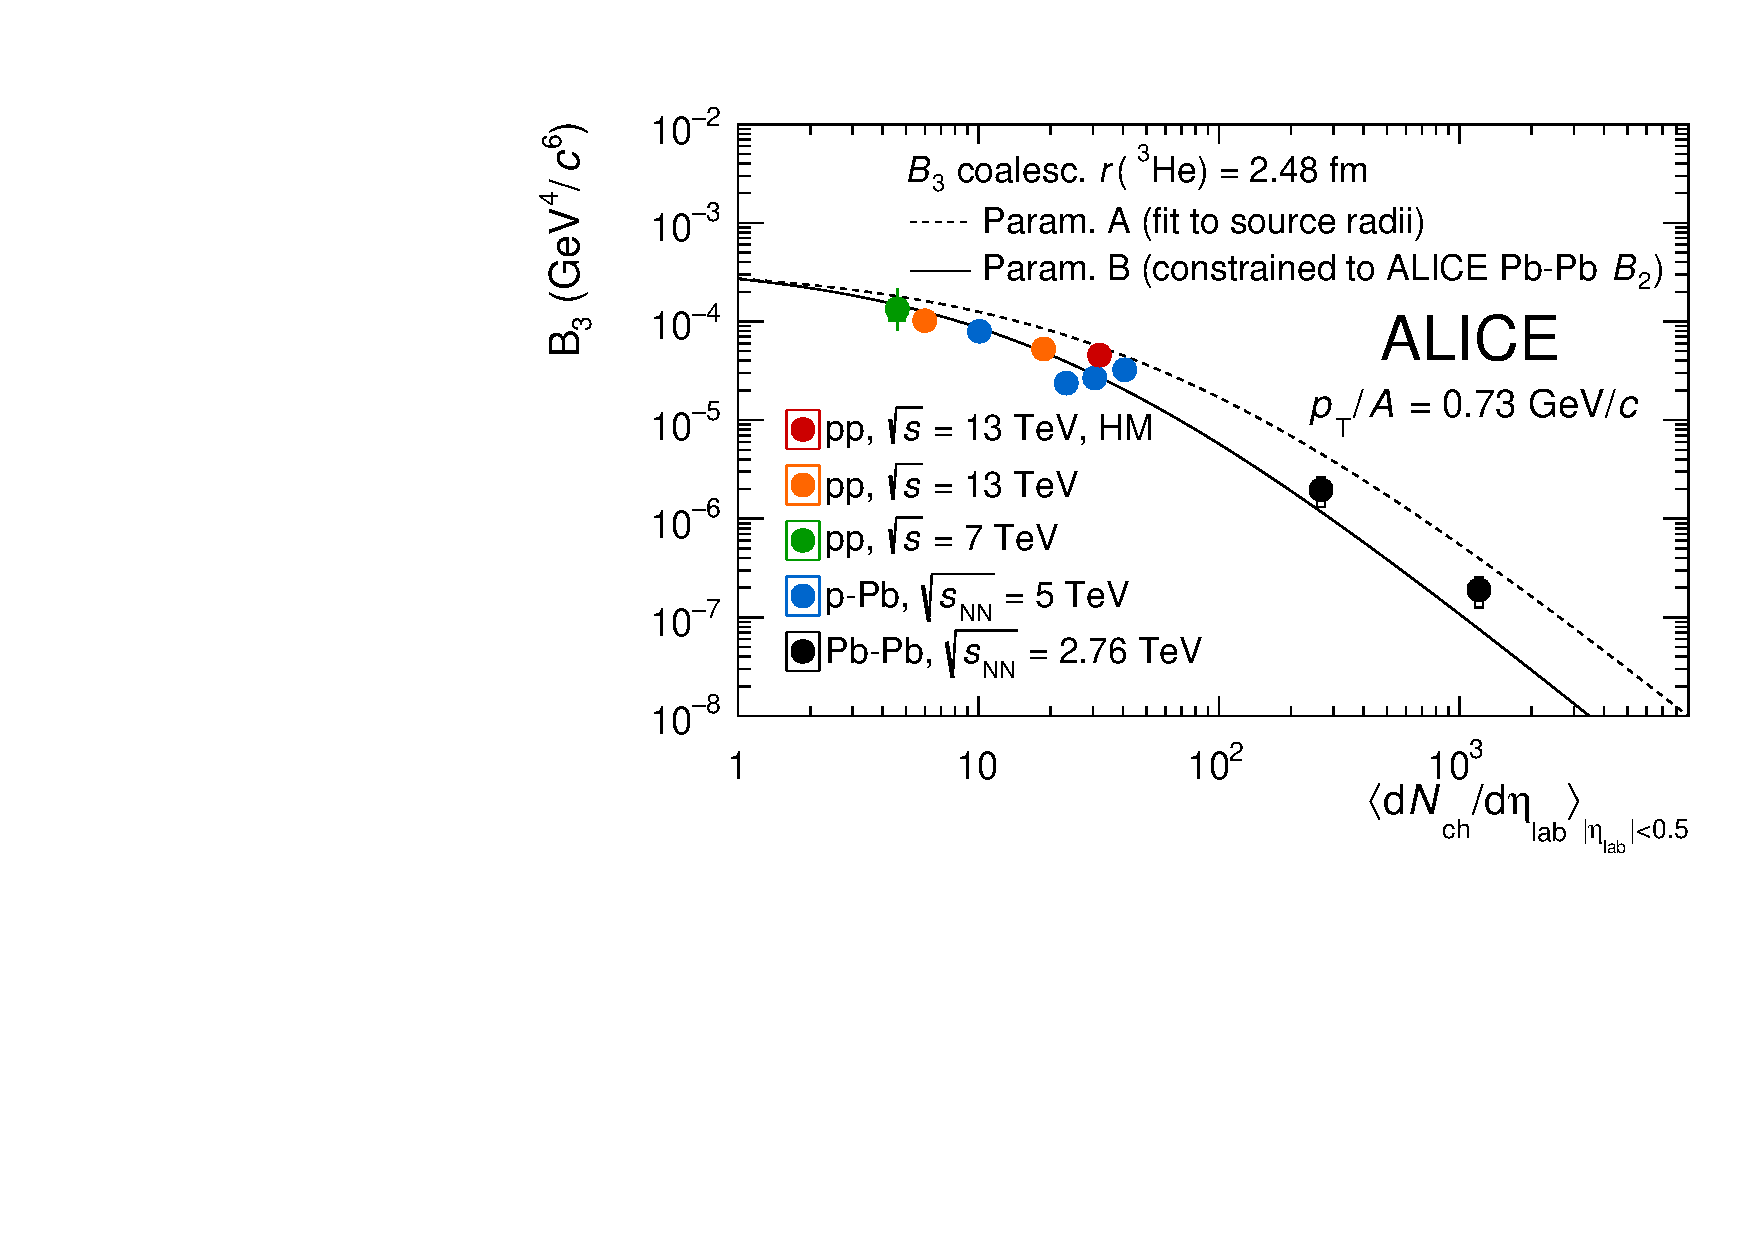
\includegraphics[width=\textwidth]{image/2-modelli/cB3vsMult.pdf}
        \caption{(Anti)elio}
        \label{fig:cB3vsMult}
    \end{subfigure}
    \captionwithsource{Misure (punti colorati) di \emph{\rmfamily (a)} $B_2$ e di \emph{\rmfamily (b)} $B_3$ in funzione della molteplicità effettuate a $p_t/A$ indicate. Le linee rappresentano le previsioni teoriche basate su due diversi parametrizzazioni del raggio della sorgente.}{\cite{alice_2022_coal_formula}} 
    \label{fig:BAvsMult}
\end{figure}
Si osserva che per la misura del parametro $B_2$, nelle collisioni a basse molteplicità (pp e p-Pb) $B_2$ ha una dipendenza debole della molteplicità, mentre per collisioni ad alta molteplicità (Pb-Pb) i dati mostrano un calo sostanziale di $B_2$. 
Analogamente per $B_3$, il modello di coalescenza descrive qualitativamente gli andamenti ma non riesce a farlo per tutto l'intervallo di molteplicità.
%%%%%%%%%%%%%%%%%%%%%%%%%%%%%%%%%%%%%%%
\section{Il modello di adronizzazione statistica}
I \emph{modelli di adronizzazione statistica} (SHM), chiamati anche modelli termici-statistici, sono utilizzati per predire l'abbondanza delle diverse specie di particelle prodotte nelle collisioni di particelle.
Questi modelli assumono che le particelle vengano emesse da una sorgente in equilibrio termico e chimico e che ogni tipo di particella abbia la possibilità di essere prodotta, purché vengano rispettate le leggi di conservazione previste dal Modello Standard.
Le abbondanze relative delle specie che vengono prodotte tuttavia verranno regolate dalle leggi della meccanica statistica, in particolare dipenderanno fortemente dalla funzione di partizione, la quale a sua volta dipenderà dal mezzo in cui avviene la collisione.
Il mezzo che si considera in questo caso è quello di un gas in espansione, non interagente, composto da particelle e risonanze, che chiamiamo \emph{Gas di Risonanze Adroniche} (HRG).
A seconda del sistema  considerato abbiamo due casi principali: se il volume di interazione è sufficientemente grande (per esempio nelle collisioni di ioni pesanti) si utilizza allora il modello statistico con un ensemble gran canonico; mentre se il volume è ridotto allora si utilizza il modello statistico nell'ensemble canonico.\\

Nel formalismo dell'ensemble gran canonico si prevede un sistema che interagisce con un reservoir, scambiando con esso energia e particelle.
Il sistema che si considera in questo caso è la regione misurabile dai rilevatori di ALICE, in contatto con il reservoir che si forma quando vi è una collisione di ioni pesanti, ossia l'HRG (non il Quark-Gluon Plasma perché esso non è invece accessibile dai rilevatori).
Assumendo che vi sia un equilibrio tra la regione e il reservoir, allora ciò implica una conservazione in media dell'energia e delle principali grandezze quantistiche, come la carica e i numeri quantici.
Quindi si utilizza il formalismo gran canonico per ottenere le proprietà statistiche di questi sistemi fisici.
Per far ciò si utilizza la funzione di partizione $Z$ e sapendo che dipende da queste proprietà, possiamo assumere che $Z = Z(T,V,\mu)$, con $T$ la temperatura del mezzo, $V$ il volume, $\mu$ il potenziale chimico collettivo definito come $\mu = \sum_iQ_i\mu_i$, con $\mu_i$ i potenziali chimici relativi a ogni carica conservata $Q_i$.
Nel reservoir, le principali grandezze che vengono conservate sono la carica elettrica $Q$, la stranezza $S$ e il numero barionico $B$.
La funzione gran canonica, data la non-interazione tra le particelle, può essere considerata come prodotto delle funzioni di partizione di singolo stato di particella,
\begin{gather}
    Z(T,V,\mu) = \prod_i Z_i(T,V,\mu_i)\\
    \implies \log Z(T,V,\mu)= \sum_i \log Z_i(T,V,\mu_i)
\end{gather}
Si può dimostrare che la funzione che descrive $\log Z_i$ ha la seguente espressione
\begin{equation}
    \log Z_i(T,V,\mu_i) = \dfrac{Vg_i}{2\pi\beta\pi^2}\sum_{k=1}^\infty \dfrac{(\pm 1)^{k+1}}{k^2}\lambda_i^k m_i^2 \ K_2(k\beta m_i) 
\end{equation}
con $g_i$ la molteplicità spin-isospin della particella nello stato $i$, $m_i$ è la sua massa, $K_2$ la funzione modificata di Bessel del secondo tipo; il termine $\pm$ assume valore $+1$ per particelle descritte dalla statistica di Bose-Einstein e $-1$ per le particelle descritte dalla statistica di Fermi-Dirac.
Una quantità interessante da ricavare è il numero medio di particelle di uno stato $i$, ottenibile da
\begin{equation}\label{eq:mean_n}
    \lrangle{N_i}_\text{th}(T,V,\mu) = \dfrac1\beta\pd{}{\mu_i} \log Z_i(T,V,\mu_i)
\end{equation}
Tuttavia questa descrizione è incompleta dal momento in cui non si è tenuto conto di contributi da parte degli stati di risonanza.
Facendo così si ottiene il numero medio totale di particelle dello stato $i$ come
\begin{equation}
    \lrangle{N_i}_\text{tot}(T,V,\mu) = \lrangle{N_i}_\text{th}(T,V,\mu) + \sum_j \Gamma_{j\to i}\lrangle{N_i}_\text{th}(T,V,\mu)
\end{equation}
con $\Gamma_{j\to i}$ il coefficiente del contributo della risonanza $j$ che decade in $i$.
Quindi il numero medio delle particelle dipende principalmente da cinque parametri, ossia la temperatura, il volume e i tre potenziali chimici.\\

Il modello di adronizzazione statistica canonica (CSM) invece riguarda volumi di interazioni minori ottenuti per esempio in collisioni pp.
Essendo il volume di interazione ridotto, allora la conservazione delle cariche non può essere più assunta in media, ma deve essere esatta, ossia senza fluttuazioni.
Questo significa che il numero di particelle cariche è soppresso rispetto a quello del modello gran canonico, per questo viene dato il nome di \emph{soppressione canonica}.
La trattazione del modello canonico è simile a quello gran canonico: si assume il HRG in equilibrio termico come sistema, caratterizzato da un volume e temperatura, con le cariche conservate ($Q$, $B$ e $S$).
Un fattore aggiuntivo da tenere in considerazione rispetto alla trattazione gran canonica in questo caso è il \emph{fattore chimico}, il quale assicura la conservazione della carica locale.
Uno degli effetti della soppressione canonica è la riduzione della produzione delle particelle con stranezza.\\

\subsection{Predizioni del SHM}
Tramite il modello SHM sono possibili diverse predizioni:
\begin{itemize}
    \item predizioni della produzione di adroni dotati di una massa variabile in una vasto intervallo di valori, si parla da pioni fino ai (anti)nuclei come l'$^{4}{\rm He}$.
    In \autoref{fig:mass_yield} si può osservare che il modello è preciso nella predizione per i nuclei, mentre tende a sottostimare leggermente la produzione degli adroni più leggeri se non si considera il contributo dovuto ai decadimenti degli stati risonanti.
    Questi non contribuiscono significativamente alla produzione di particelle massive come i nuclei.
\begin{figure}[htpb]
    \centering
    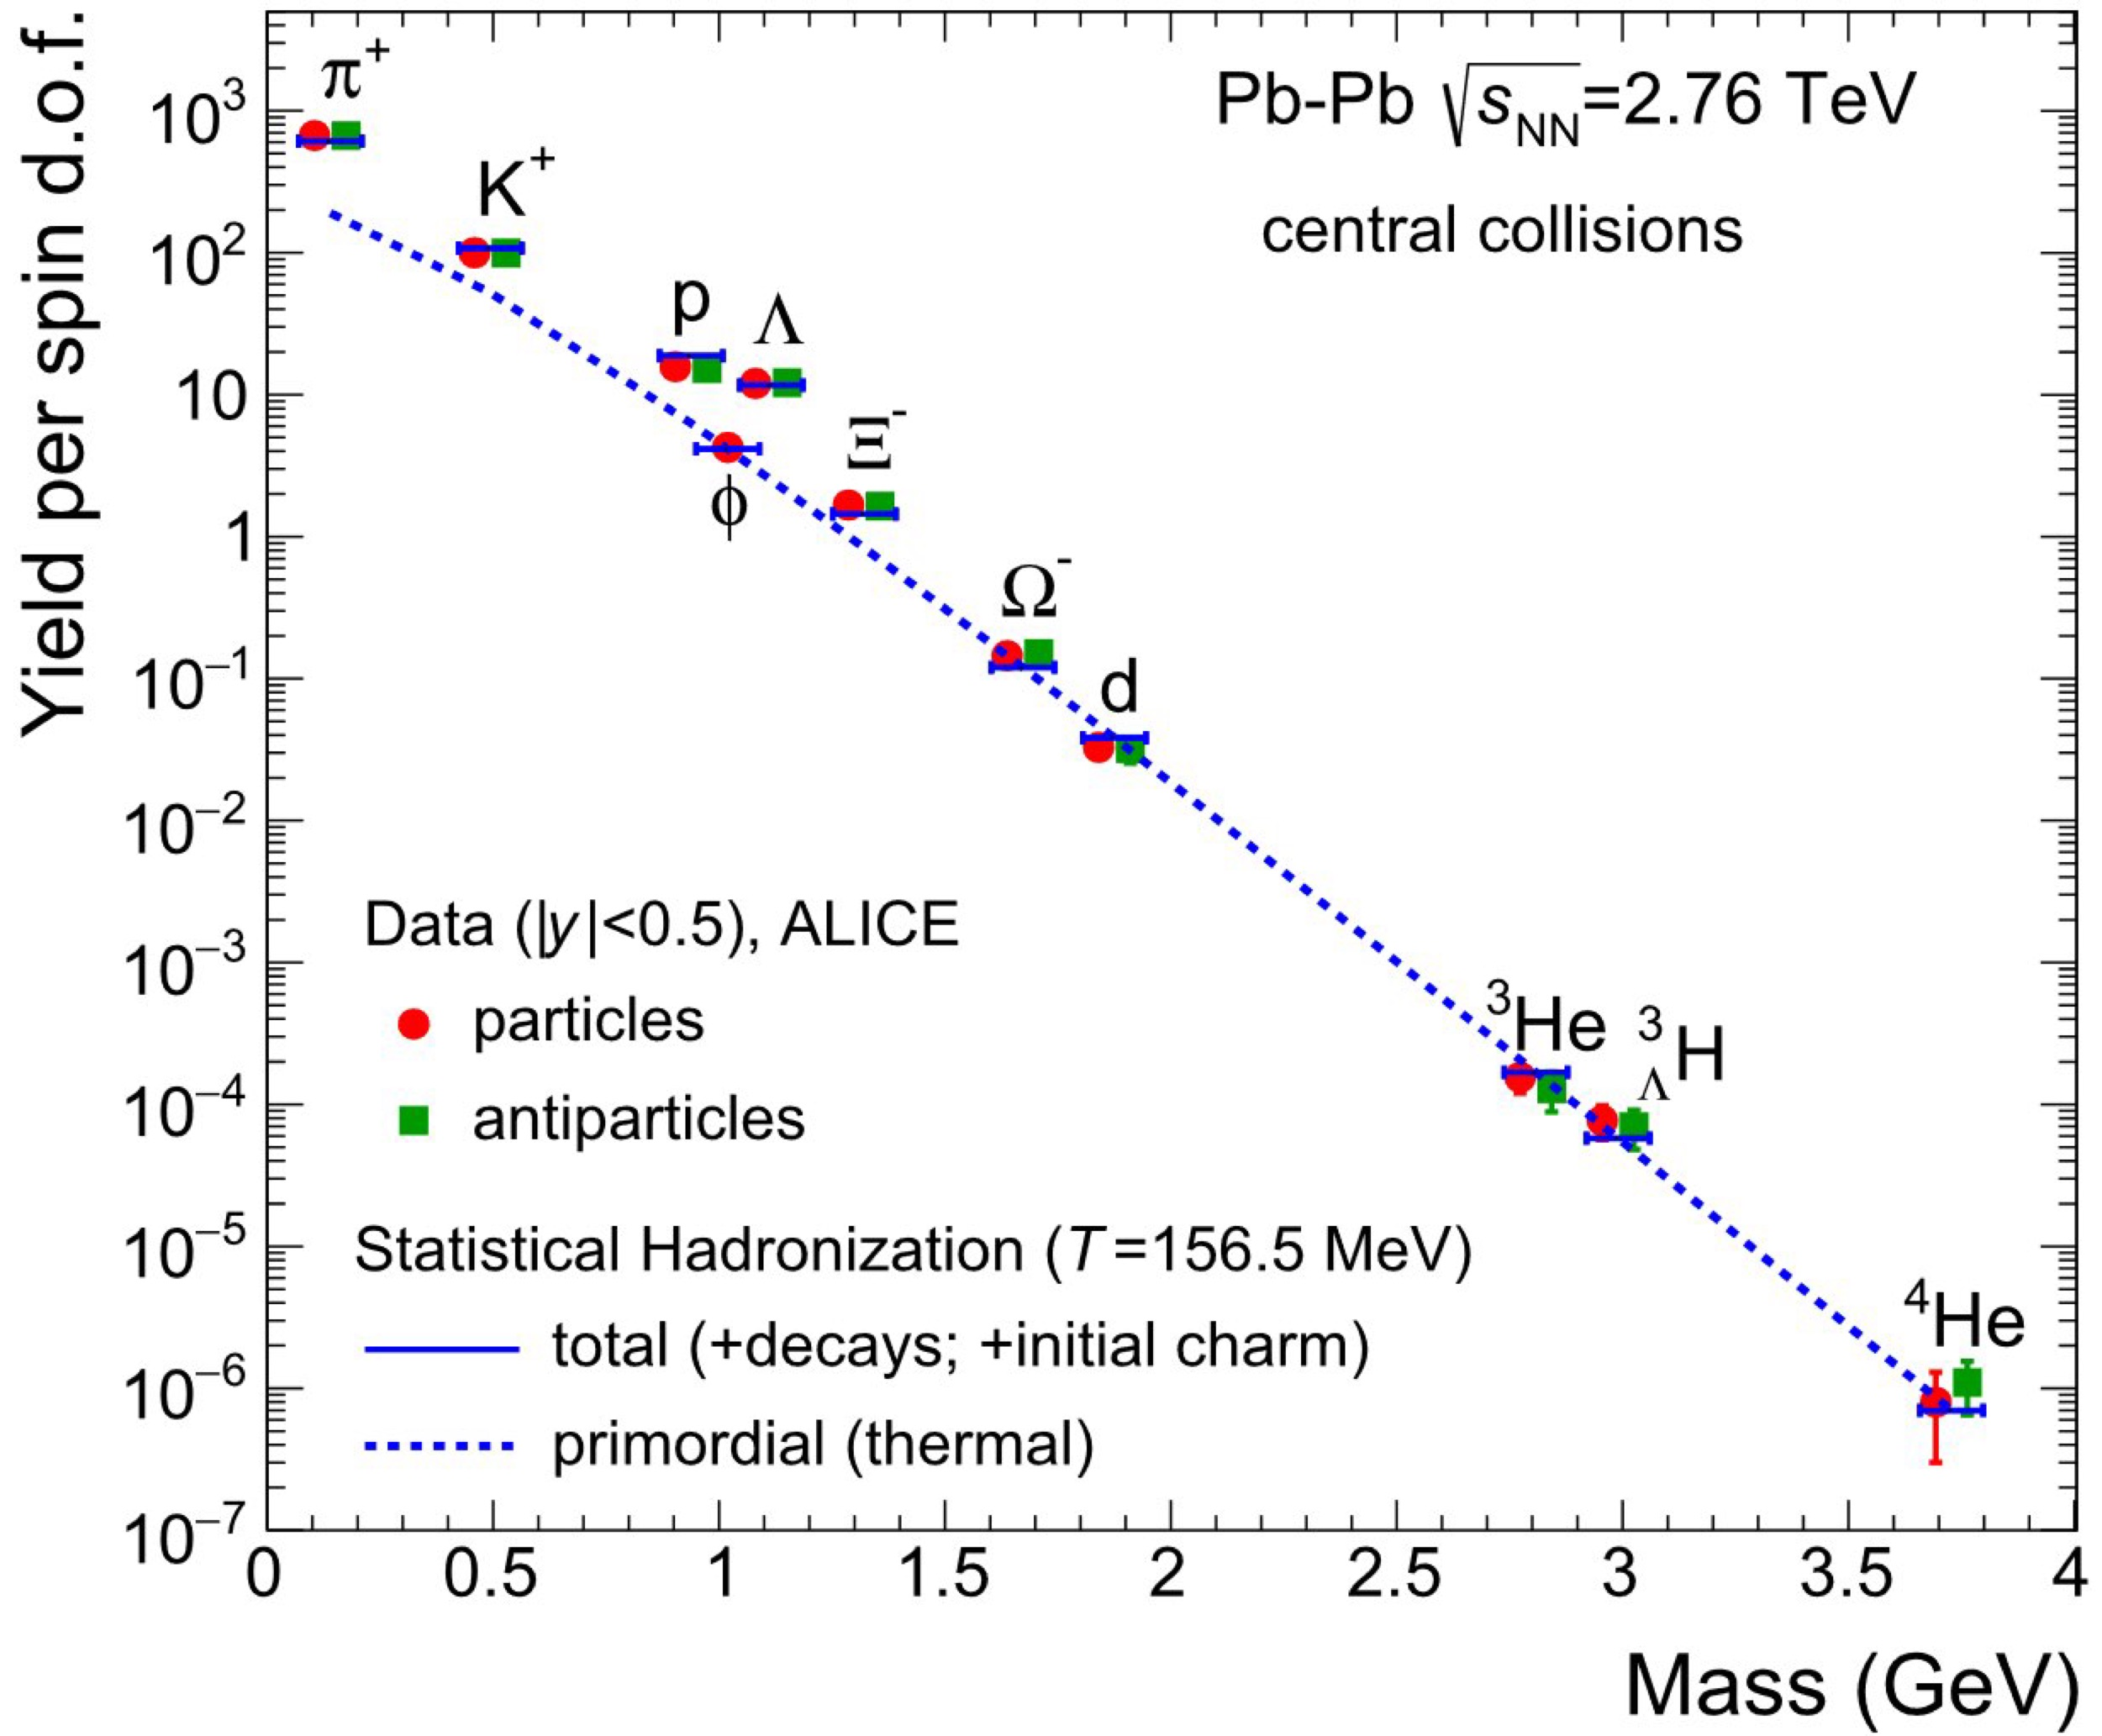
\includegraphics[width=0.6\linewidth]{image/2-modelli/mass_yield.jpg}
    \captionwithsource{(Linea tratteggiata) Variazione della produzione delle (anti)particelle rispetto alla rapidità (normalizzato  degenerazione di spin) in funzione della massa della particella, in confronto con i dati di ALICE.}{\cite{mass_yield}}
    \label{fig:mass_yield}
\end{figure}
    \item Predizioni del rapporto tra materia e antimateria in funzione dell'energia della coppia di nucleoni.
    Si può osservare come per valori piccoli dell'energia di collisione ($\sim$ 100 GeV), il potenziale barionico, una misura del rapporto materia-antimateria, assuma valori alti, per poi tendere a zero con l'aumentare dell'energia del sistema.
    Questo è compatibile con ciò che si osserva in LHC (\autoref{fig:matter_antimatter}) in cui la simmetria tra materia e antimateria è praticamente ottenuta \cite{Tawfik_2011_matter_antimatter}.
\end{itemize}
\begin{figure}[htbp]
    \centering
    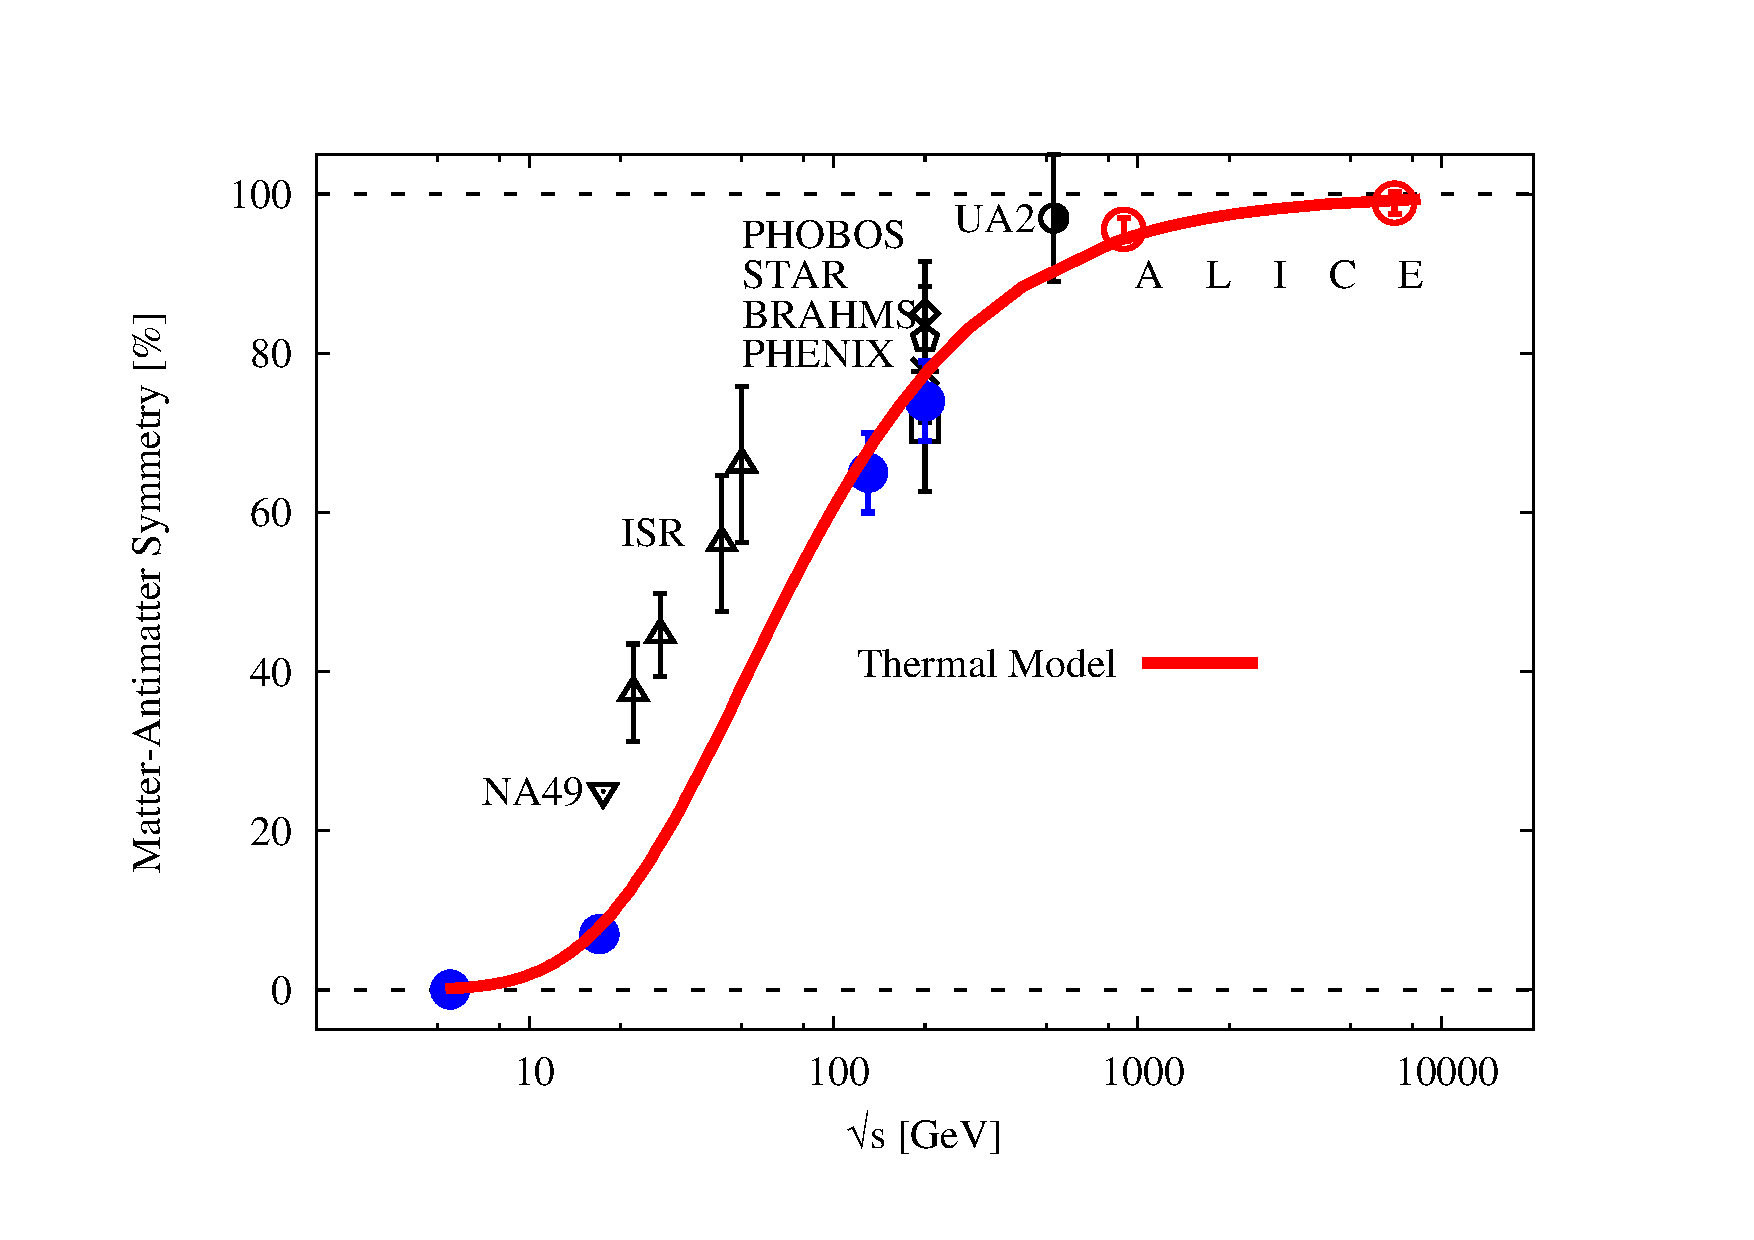
\includegraphics[width=0.8\linewidth]{image/2-modelli/antiPP_Alice2010_2.pdf}
    \captionwithsource{Rapporti di ${\bar{p}}/p$ in funzione dell'energia del centro di massa $\sqrt{s}$. I simboli vuoti indicano i risultati da vari esperimenti di collisioni pp, mentre i simboli pieni rappresentano quelli da collisioni di ioni pesanti. La curva nera rappresenta le previsioni del modello termico sul rapporto $\bar p/p$ del SMH.}{\cite{Tawfik_2011_matter_antimatter}}
    \label{fig:matter_antimatter}
\end{figure}
\section{Confronto del modello di coalescenza con il CSM}
In questa sezione si esegue un confronto tra il modello di coalescenza e il modello di adronizzazione statistica canonica.
Per far ciò confrontiamo i modelli teorici con dati sperimentali riguardo alle misure di rapporti di produzione tra nuclei e protoni in funzione della molteplicità \cite{alice_2022_coal_formula}.
Più specificatamente si vanno a considerare i rapporti $(D+\bar D)/(p + \bar p)$ e $(^3\text{He} + ^3\overline{\text{He}})/(p+\bar p)$.
I grafici prodotti sono riportati in \autoref{fig:NoPvsMult}.
Per le previsioni del CSM utilizza il pacchetto software del \ttbox{Thermal-FIST} \cite{Vovchenko_2019_thermal_FIST}, utilizzando dei volumi di correlazione $V_C$ tra 1 e 3 unità di rapidità.
Invece, per il modello di coalescenza si utilizza l'implementazione effettuata in \cite{Sun_2019_coal_model}.
È importante notare che si sono utilizzati due modelli di coalescenza per il nucleo di (anti)$^{3}{\rm He}$: il modello di coalescenza a tre corpi, in cui si assume la formazione del nucleo a partire dalla vicinanza di due protoni e di un neutrone; il modello a due corpi, in cui si assume la formazione del nucleo a partire da un (anti)deuterone e un (anti)neutrone. 
\begin{figure}[h]
    \centering
    \begin{subfigure}{.49\textwidth}
    \centering
        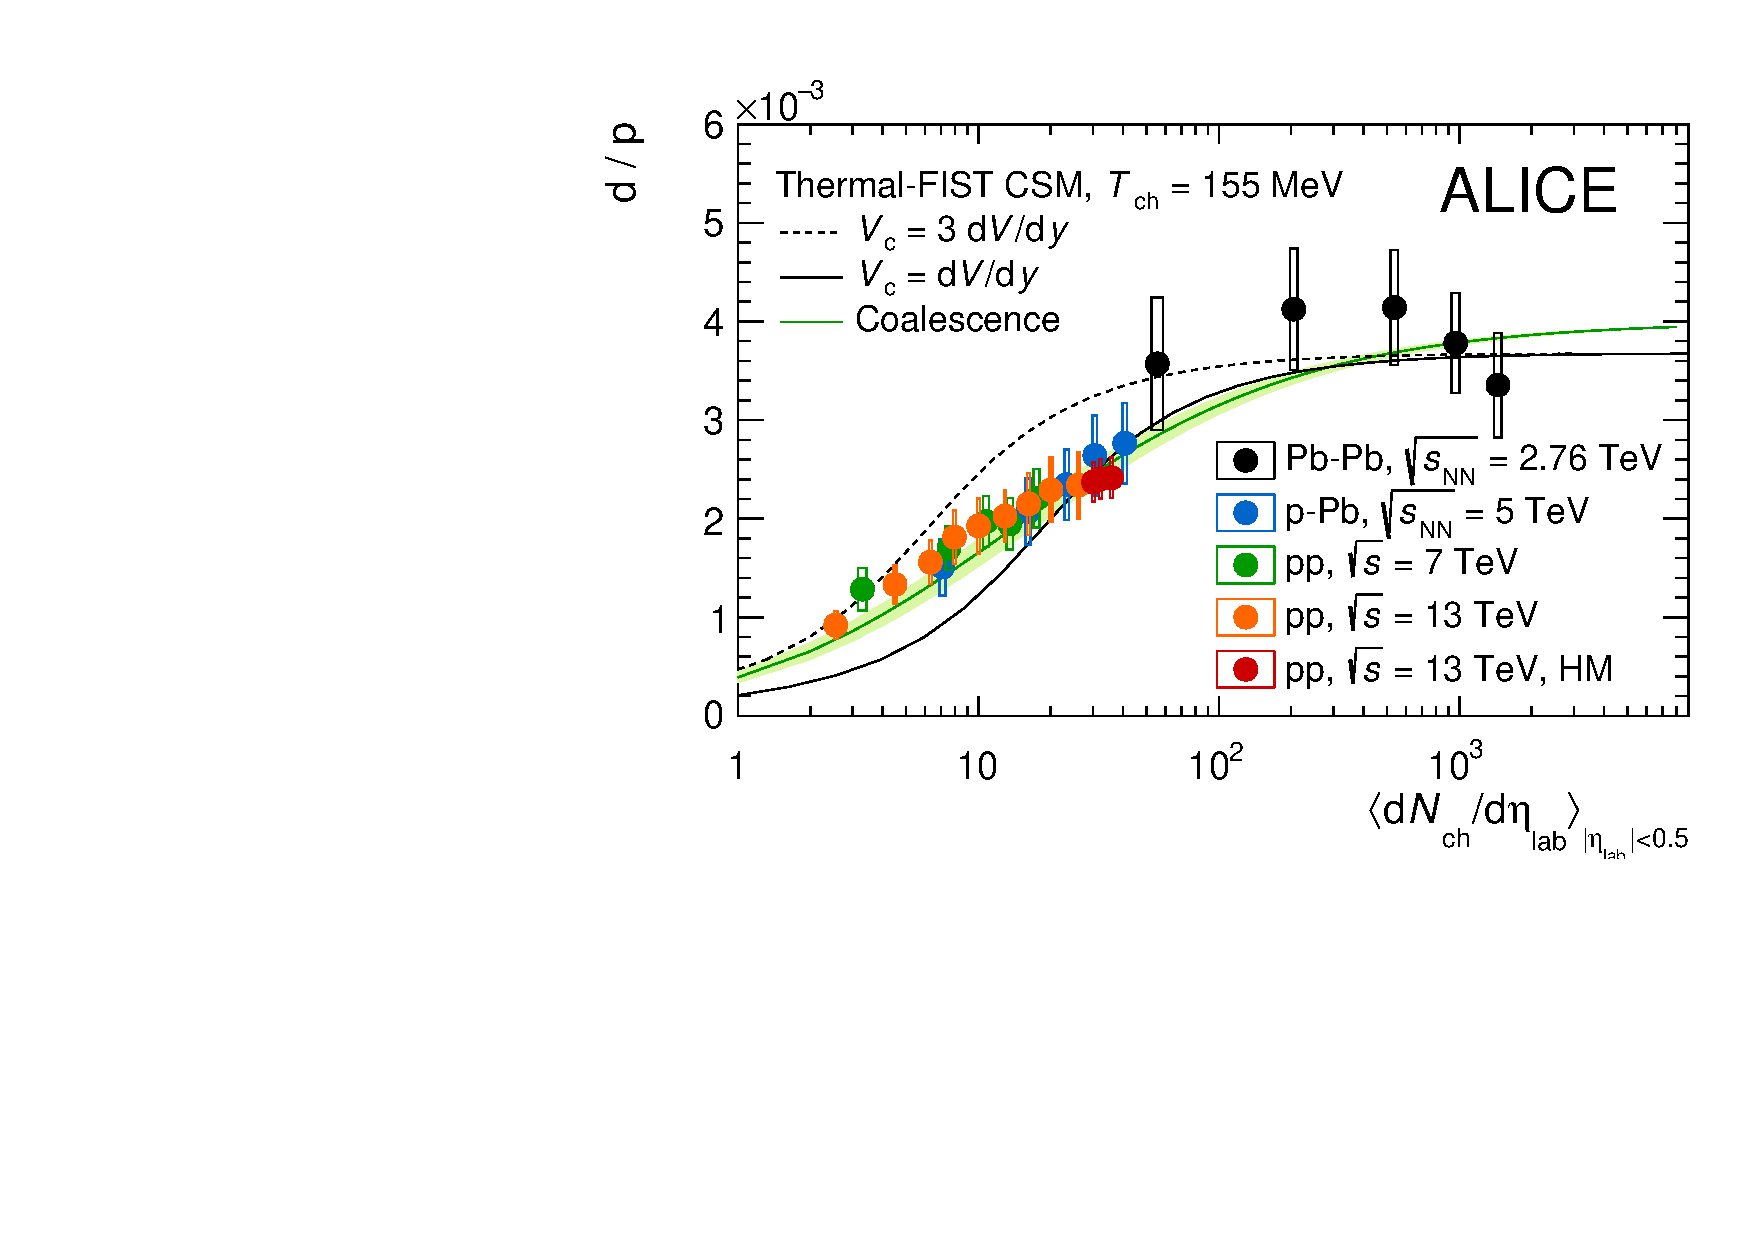
\includegraphics[width=\textwidth]{image/2-modelli/cDoPvsMult.pdf}
        \caption{$(D+\bar D)/(p + \bar p)$}
        \label{fig:cDoPvsMult}
    \end{subfigure}
    %\hspace{1cm}
    \begin{subfigure}{.49\textwidth}
        \centering
        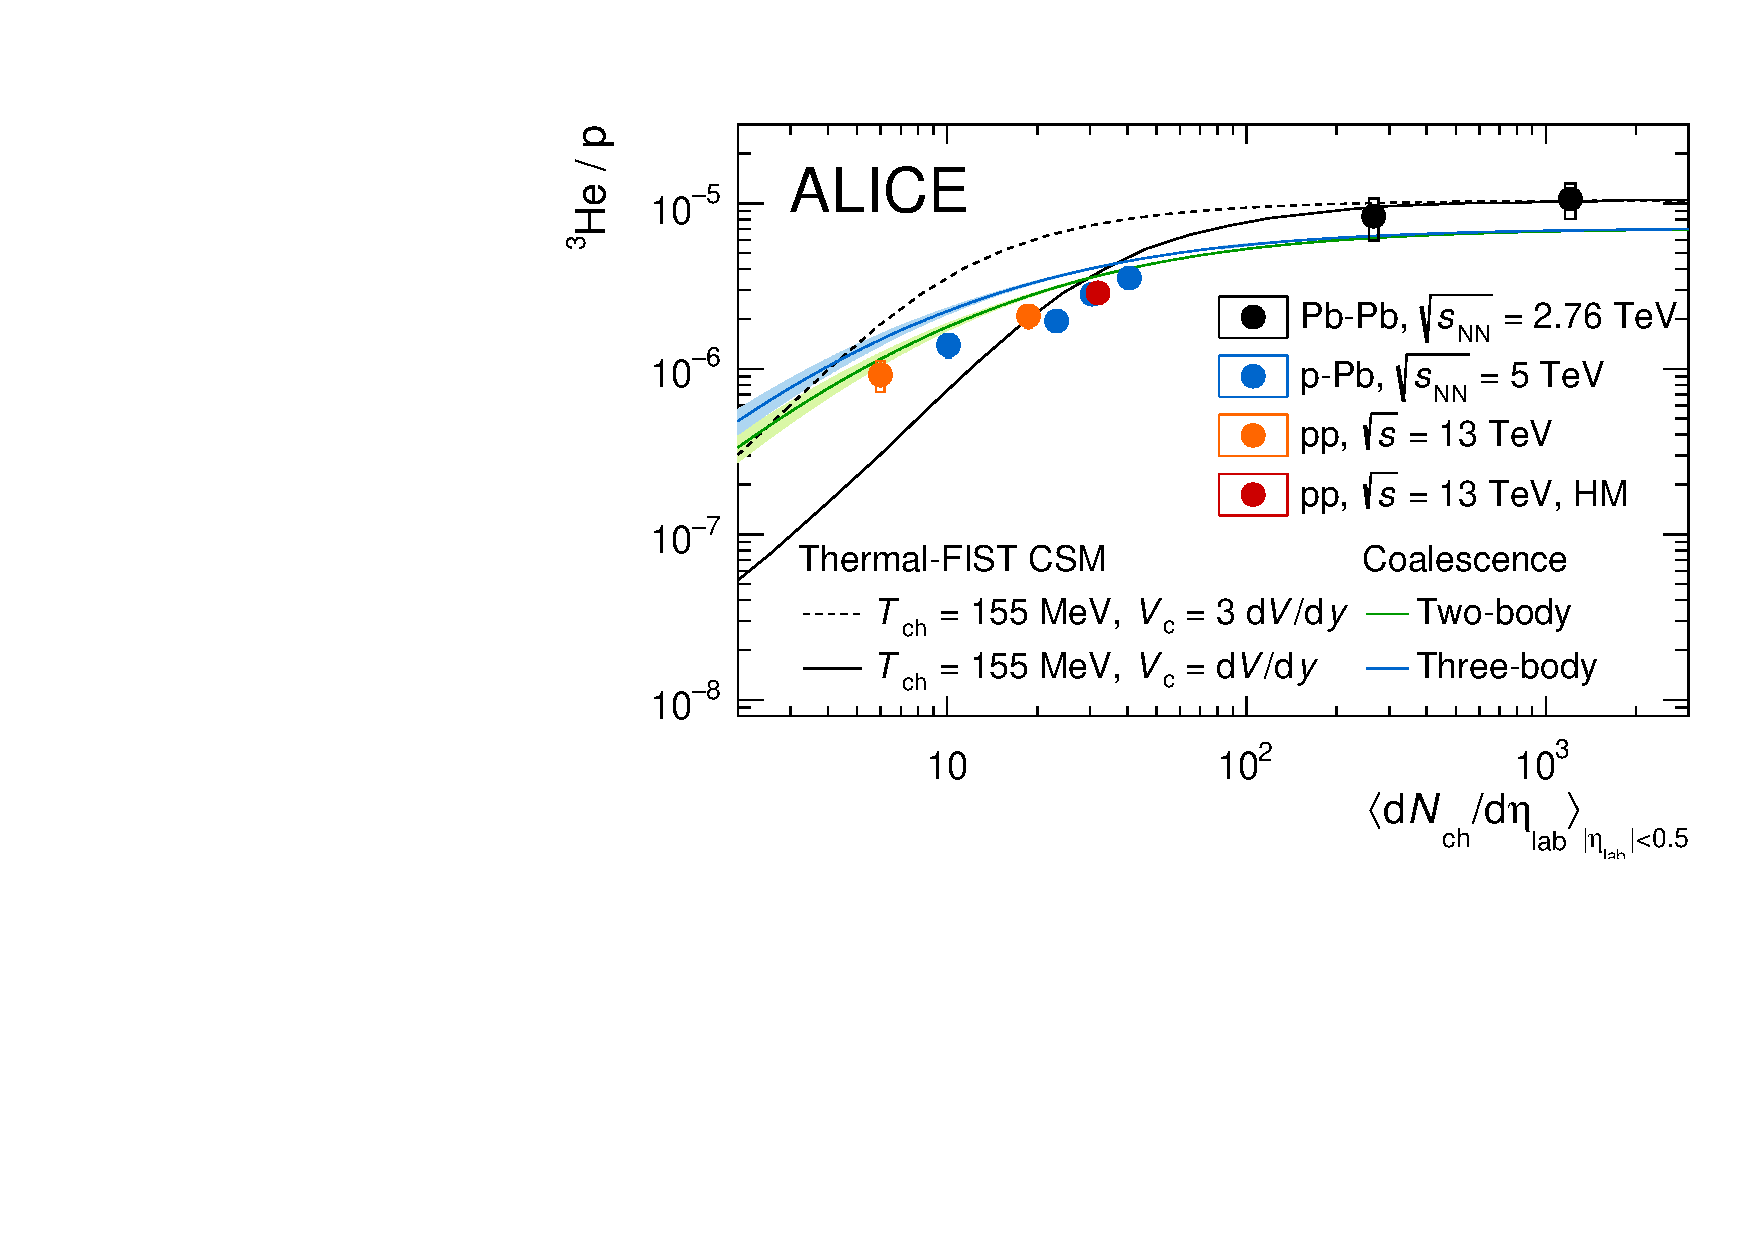
\includegraphics[width=\textwidth]{image/2-modelli/cHEoPvsMult.pdf}
        \caption{$(^3\text{He} + ^3\overline{\text{He}})/(p+\bar p)$}
        \label{fig:cHEoPvsMult}
    \end{subfigure}
    \captionwithsource{Misure (punti colorati) dei rapporti tra la produzione dei nuclei e protoni in funzione della molteplicità per \emph{\rmfamily (a)} (anti)deuteroni e \emph{\rmfamily (b)} (anti)nuclei di $^3\text{He}$. Le linee nere continue e tratteggiate rappresentano le previsioni del \emph{\ttbox{Thermal-FIST}} CSM.
    "$d/p$" indica $(D+\bar D)/(p + \bar p)$ e "$^3\text{He}/p$" indica $(^3\text{He} + ^3\overline{\text{He}})/(p+\bar p)$.
    In \emph{\rmfamily (a)} la linea verde rappresenta il modello di coalescenza, in \emph{\rmfamily (b)} la linea verde e blu rappresentano rispettivamente il modello di coalescenza a due corpi e a tre corpi.}{\cite{alice_2022_coal_formula}} 
    \label{fig:NoPvsMult}
\end{figure}

Per quanto riguarda le misure sperimentali, esse sono consistenti con esperimenti effettuati in passato \cite{Adam_2016_a1, 2017_a2, Acharya_2018_a3}: gli andamenti dei due rapporti aumentano con l'aumentare della molteplicità e i valori si saturano ad alte molteplicità.
Per quanto riguarda invece le previsioni teoriche, solamente il modello di coalescenza sembra essere qualitativamente in accordo con i dati, per entrambi i rapporti.
In particolare per $D/p$, il modello di coalescenza riesce a riprodurre fedelmente i dati per tutto l'intervallo della molteplicità, mentre per $^3\text{He}$ abbiamo una migliore concordanza del modello di coalescenza a due corpi nelle regioni a bassa bassa molteplicità, mentre ad alte molteplicità (come per le misure delle collisioni Pb-Pb) si ha un discostamento maggiore.
Il modello statistico canonico fornisce invece un andamento più qualitativo per molteplicità più basse, mentre ha un andamento consistente con i dati nel regime del gran-canonico (ossia nelle molteplicità caratterizzate dagli urti Pb-Pb).
\section{PYTHIA 8.3}
\pythiaa{} \cite{pythia8300} è un generatore Monte Carlo utilizzato principalmente per la generazione di eventi di collisione di particelle nella fisica delle alte energie. 
Più in particolare esso riesce a riprodurre processi QCD utilizzando sia implementazioni teoriche che fenomenologiche, dove i parametri sono determinati a partire da dati sperimentali. 
L'utilizzo di \pythiaa{} può essere utile in molteplici campi, per esempio la maggior parte della base degli utenti proviene dalle grandi collaborazioni di LHC, ma anche in fisica astroparticellare oppure nucleare.

Per evento di collisione si intende l'insieme degli avvenimenti che comprendono le particelle iniziali, le particelle finali e tutte le particelle e risonanze intermedie.
La ripetizione nella generazione di questi eventi deve essere necessariamente resa casuale, data l'imprevedibilità dei processi quanto-meccanici.
La generazione dipende da parametri che vengono impostati nel software che possono essere modificati a piacimento dall'utente a seconda delle proprie esigenze.

\subsection{Struttura del programma}
% struttura di programma
In un vero evento di collisione di particelle vi sono numerosi processi QCD, QED e altri che sono noti per essere molto complessi, perciò è logico andare a ordinarli e raggrupparli secondo un criterio temporale o in termini di energie.
Per esempio in \cite{pythia8300} si prende come esempio un evento $pp\to t\bar t$ e si ordinano gli eventi secondo una logica in termini dell'\textit{hardness} dei processi:
si parte con uno scattering inelastico di partoni, seguito dalla produzione di risonanze (bosoni deboli o quark top), con aggiunta di correzioni radiative.
Successivamente si hanno radiazioni dello stato iniziale (ISR), e dello stato finale (FSR), originati dal decadimento delle particelle iniziali e dalle risonanze rispettivamente.
Queste radiazioni sono sostanzialmente sciami (o cascate) di partoni.
Contestualmente a ciò vi sono interazioni multi-partoniche (MPI), ulteriori processi di scattering, in aggiunta ad altri processi QCD che esulano dalla trattazione di questa tesi. 
Infine verso la fine del processo si formano gli adroni stabili a partire da decadimenti dei partoni instabili.
Una rappresentazione grafica di tutti questi processi è riportata in \autoref{fig:eventSchematic}.

\begin{figure}[htpb]
\centering % 73% + 27%
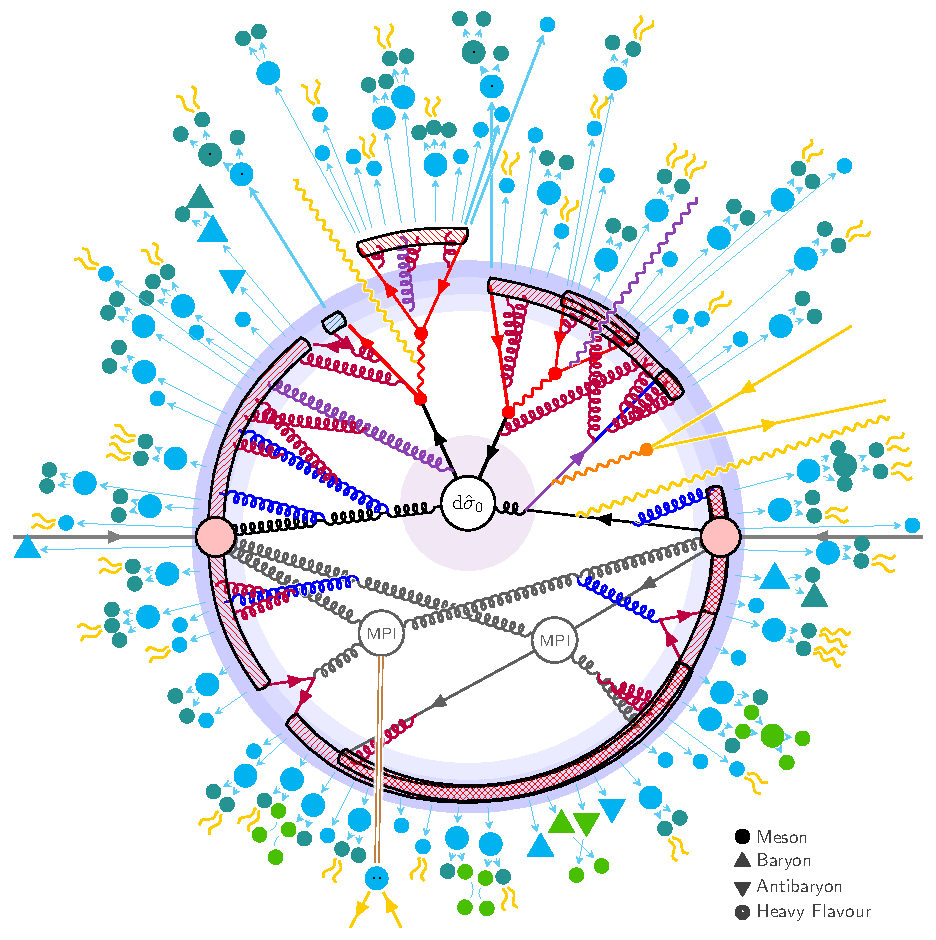
\includegraphics[width=0.73\textwidth]{image/2-modelli/event.pdf}%
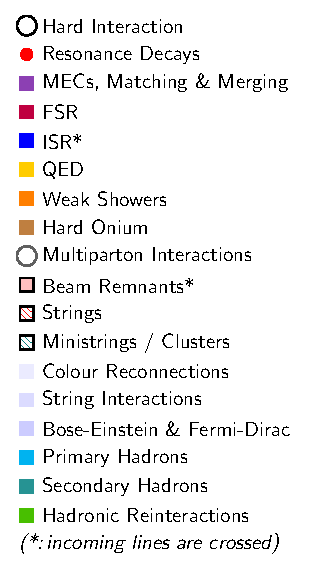
\includegraphics[width=0.27\textwidth]{image/2-modelli/eventLegend.pdf}
\captionwithsource{Schematica (semplificata) di un evento $pp\to t\bar t$ nel modello di \emph{\pythiaa{}}.
Le particelle entranti sono rappresentate dalle linee grigie esterne a metà altezza.  
\label{fig:eventSchematic}}{\cite{pythia8300}}
\end{figure}

\pythiaa{}, ispirandosi a questo modo di trattare un evento, è suddivisa in tre parti principali:
\begin{enumerate}
    \item \emph{livello di processo}, corrispettivo del processo di scattering duro, dove vengono prodotte anche le risonanze;
    \item \emph{livello di partoni}, dove vengono gestite le ISR e le FSR tramite l'implementazione di modelli di sciami partonici, le MPI e varie correzioni QCD;
    \item \emph{livello di adroni}, durante la quale viene gestita l'adronizzazione in senso stretto, tramite decadimenti di adroni e risonanze instabili e altri processi più tecnici.
\end{enumerate}
Ovviamente questi livelli non sono gestiti in maniera totalmente separata, ma vi è un numero significativo di oggetti condivisi da un livello all'altro.

% https://amzn.eu/d/6InjjKU per giovanni

\subsection{Gli algoritmi di generazione}
%%%%%%%%%%
Gli algoritmi di generazione in \pythiaa{} si basano su numeri pseudo-casuali campionati da distribuzioni di probabilità, simulando la natura stocastica degli eventi reali nelle collisioni di particelle.
In seguito vengono elencate le due principali utilizzate nel programma.
\begin{itemize}
    \item \emph{Algoritmo di veto}, il principale algoritmo di \pythiaa{} per simulare processi come decadimenti radiativi, cascate partoniche o interazioni multi-partoniche (MPI).
    Il suo funzionamento è semplice: partendo da una funzione di prova che sovrastima la distribuzione di probabilità desiderata, vengono generati dei campioni e viene deciso se sono conformi alla probabilità voluta, e in base a ciò viene deciso se la funzione di prova sia accettabile o se vi sia bisogno di ripetere questo step.
    Esistono inoltre anche varianti di questo algoritmo;
    % aggiungere altro se serve
    \item vi sono algoritmi per la distribuzione uniforme della quantità di moto nello spazio delle fasi.
    Nel caso di due particelle questo è triviale, in quanto è sufficiente emetterle in direzioni opposte nello spazio dei momenti.
    Mentre per tre o più particelle prodotte vengono utilizzate principalmente \emph{M-generator} e \emph{RAMBO}.
    Quest'ultimo è la migliore scelta per i prodotti senza massa (o massa trascurabile).
    \textit{M-generator} funziona scomponendo un processo di produzione  multiparticellare in produzione di 2 particelle.
    Per esempio un processo $0\to1234$ viene scomposto in $0\to(123) + 4$ e così via.
\end{itemize}
In generale, per ogni processo in \pythiaa{} è spesso implementata una forma derivata da uno di questi due principali algoritmi.   

\subsection{Formazione di deuteroni in PYTHIA} \label{ch:pythia_deuteron}
\pythiaa{} supporta la produzione deuteronica tramite due modelli di produzione, ovvero il modello di coalescenza e il modello di sezioni d'urto efficaci, chiamato anche modello di Dal-Raklev \cite{Dal_2015}, con quest'ultimo come opzione predefinita di \pythiaa{}.
Si noti come in questo paragrafo, per evitare ripetizioni, si tratterà solamente della produzione dei deuteroni, invece la trattazione degli antideuteroni è equivalente nel momento in cui si considerano le antiparticelle corrispettive.

\subsubsection{Modello di coalescenza}
Il modello di coalescenza, come già detto in precedenza, prevede la formazione di un deuterone nel momento in cui un protone e un neutrone sono sufficientemente vicini nello spazio delle fasi.
L'implementazione di questo modello in \pythiaa{} è effettuata in questo modo: vengono prese in considerazione tutte le coppie possibili di protoni e neutroni $p-n$ e si considera per ognuna di esse il modulo della differenza della loro quantità di moto (calcolato nel sistema di centro di massa di ognuna coppia)
\begin{equation}\label{eq:momentum_difference_k}
    k = |\vec p_p - \vec p_n|
\end{equation} 
Si determina la formazione del deuterone nel momento in cui $k<p_0$, con $p_0$ un parametro da determinare sperimentalmente.
È importante notare come non vi sia considerazione delle coordinate spaziali.
Un altro elemento da tenere in conto è la violazione energetica della coalescenza, ossia che il processo $pn\to D$ non è possibile se nello stato finale non vi sia un'altra particella.
Per ovviare a questo problema si considera al posto di questa reazione la cattura radiativa, ovvero $pn\to \gamma D$, in quanto provvede a fornire un'approssimazione ragionevole del processo.
Per esprimere la probabilità di formazione del deuterone in funzione di $k$ in modo compatto si può farlo nel seguente modo
\begin{equation}
    P(k) = \theta(p_0-k)
\end{equation}
con $\theta(k)$ la funzione gradino di Heaviside.

\subsubsection{Modello di sezioni d'urto efficaci}
Nel modello di sezioni d'urto efficaci si punta a descrivere la formazione dei deuteroni da un punto di vista probabilistico, di fatto considerando la probabilità di formazione $P_\text{processo}(k)$ direttamente proporzionale alla sezione d'urto differenziale del processo $\sigma_\text{processo}(k)$
\begin{gather}
    P_\text{processo}(k) \propto \dfrac{d\sigma_\text{processo}(k)}{dk} \\
    \implies P_\text{processo}(k) = \dfrac1{\sigma_0}\dfrac{d\sigma_\text{processo}(k)}{dk} 
\end{gather}
con $k$ la grandezza definita dell'\autoref{eq:momentum_difference_k} e $\sigma _0$ una costante di proporzionalità da determinare sperimentalmente, analogo di $p_0$.
L'obiettivo del modello di sezioni d'urto efficaci è anche quello di uniformare questo parametro in modo che sia costante in tutti gli esperimenti, al contrario di $p_0$ che assume valori diversi in esperimenti diversi. 

A differenza del modello di coalescenza, in questo modello non si considera solamente la reazione della cattura radiattiva, ma se ne considerano molteplici.
I canali di produzione dei deuteroni sono riportati in \autoref{tab:canali}.

\begin{table}[H]
    \centering
    \begin{tabular}{clcl}
    \hline \hline
    1) & $pn \to \gamma D$ & 5) & $pp \to \pi^+ D$\\
    2) & $pn \to \pi^0 D$ & 6) & $pp \to \pi^+\pi^0 D$\\
    3) & $pn \to \pi^-\pi^+ D$ & 7) & $nn \to \pi^- D$\\
    4) & $pn \to \pi^0\pi^0 D$ & 8) & $nn \to \pi^-\pi^0 D$\\
    \hline\hline
    \end{tabular}
    \caption{I canali di produzione dei deuteroni considerati nel modello di sezione d'urto. Per ottenere i canali dell'antideuterone è sufficiente considerare le antiparticelle.}
    \label{tab:canali}
\end{table}
Ognuno di questi canali ha una propria probabilità di formazione, determinata non più come una semplice distribuzione uniforme con cut-off come nel modello di coalescenza, ma determinata da fit di dati sperimentali sullo scattering differenziale di nucleoni.

Le possibili funzioni di sezioni d'urto differenziali ${d\sigma_\text{processo}(k)}/{dk}$ sono tre:
\begin{itemize}
    \item Per $pn\to\gamma D$ è parametrizzato da un polinomio sotto a un valore $a_0$ di $k$, altrimenti da un andamento esponenziale
    \begin{equation}
        \dfrac{d\sigma(k)}{dk} =
        \begin{cases}
            \displaystyle\sum_{i=1}^{12}a_ik^{i-2} & k<a_0 \\
            e^{-c_{13}k - c_{14}k} & k>a_0
        \end{cases}
    \end{equation}
    Si assume inoltre che per $k<0.1$ GeV la sezione d'urto differenziale sia fissata al valore di $k=0.1$ GeV.

    \item Per processi che coinvolgono la formazione di un pione e di un deuterone si assume la seguente forma della sezione d'urto differenziale
    \begin{equation}
        \dfrac{d\sigma(q)}{dq} = \dfrac{c_0\ q^{c_1}}{(c_2-e^{c_3 q})^2 + c_4}
    \end{equation}
    con $q = |\vec p_\pi|/m_\pi$, con $\vec p_\pi$ la quantità di moto del pione nel centro di massa e $m_\pi$ la massa del pione.

    \item Infine per i processi di formazione di 3 corpi la sezione d'urto differenziale è parametrizzata nel seguente modo
    \begin{equation}
        \dfrac{d\sigma(k)}{dk} = \sum_{i=0}\dfrac{c_{5i}\ k^{c_{1+5i}}}{(c_{2 + 5i}-e^{c_{3 + 5i} k})^2 + c_{4 + 5i}}
    \end{equation}
\end{itemize}
La giustificazione dell'utilizzo di queste forme delle sezioni d'urto è reperibile in \cite{Dal_2015}.\\

I valori dei parametri di coalescenza ($p_0$) e di Dal-Raklev sono già stati determinati eseguendo fit ai dati sperimentali e possono essere reperiti in \cite{Dal_2015}.
In \pythiaa{}, come è già stato detto, il modello predefinito è il modello di sezioni d'urto efficaci.
Il parametro $\sigma_0$, o meglio $1/\sigma_0$, è un parametro importante perché determina il numero di deuteroni prodotti in tutti i canali di produzione. 
Tuttavia, per ragioni pratiche, in \pythiaa{} il parametro $1/\sigma_0$ è incorporato in un altro parametro, ovvero \ttbox{DeuteronProduction:norm}, che per semplicità indicheremo con \ttbox{norm}, calcolato come 
\begin{equation}\label{eq:norm}
    \ttbox{norm} = \dfrac{1}{(1/\sigma_0)(d\sigma/dk)_\text{max}}
\end{equation}
con $(d\sigma/dk)_\text{max}$ il valore della sezione d'urto differenziale massima.
Il ruolo di questo parametro è simile a quello di $1/\sigma_0$, ossia quello di regolare il numero di (anti)deuteroni prodotti per tutti i canali. Più è alto il suo valore, minore è la produzione, e viceversa.\\

Usando i parametri della tabella VI di \cite{Dal_2015} è possibile ricavare il valore massimo della sezione d'urto differenziale che è di circa $3.18$ mb.
Perciò ora per ottenere il valore di \ttbox{norm} è sufficiente conoscere il valore di $1/\sigma_0$.
Tuttavia, la determinazione di questo parametro è problematica perché varia in base all'energia del centro di massa $\sqrt s$, e in \cite{Dal_2015} sono stati ottenuti i valori di $1/\sigma_0$ e di $p_0$ che vengono riportati nella tabella VIII in \cite{Dal_2015}, in base a fit effettuati sui dati di ALICE.
Questi valori sono riportati per convenienza in \autoref{tab:valori_p0_1sigma0}.
\begin{table}[H]
    \centering
    \begin{tabular}{||c||c|c||c|c||}
    \hline \hline
    & \multicolumn{2}{c||}{$p_0$ [\si{MeV}]} & \multicolumn{2}{c||}{$1/\sigma_0$ [\si{barn^{-1}}]}\\
    \hline
    \textsc{energia} & \textsc{deuteroni} & \textsc{antideut.} & \textsc{deuteroni} & \textsc{antideut.} \\ 
    \hline
    0.9 TeV & 201 & 201 & 3.58 & 3.63\\
    2.76 TeV & 194 & 196 & 2.93 & 2.88\\
    7 TeV & 194 & 195 & 2.63 & 2.58\\
    \hline\hline
    \end{tabular}
    \captionwithsource{I valori dei parametri $p_0$ e $1/\sigma_0$ alle energie riportate. Per \emph{\rmfamily\textsc{energia}} si intende l'energia  del centro di massa $\sqrt s$.}{\cite{Dal_2015}}
    \label{tab:valori_p0_1sigma0}
\end{table}
\pythiaa{} utilizza il parametro \ttbox{norm} considerando esclusivamente il valore di $1/\sigma_0$ a 7 \si{TeV} dei deuteroni, quindi, utilizzando l'\autoref{eq:norm}, si ha che $\ttbox{norm} = 119.6$.